\documentclass[10pt]{article}
\usepackage[margin=0.7in]{geometry}
\usepackage[T1]{fontenc}
\usepackage{graphicx,hyperref}
\begin{document}
\sloppy
\section*{C-zero Cantor reduction and divisor-class derivation}
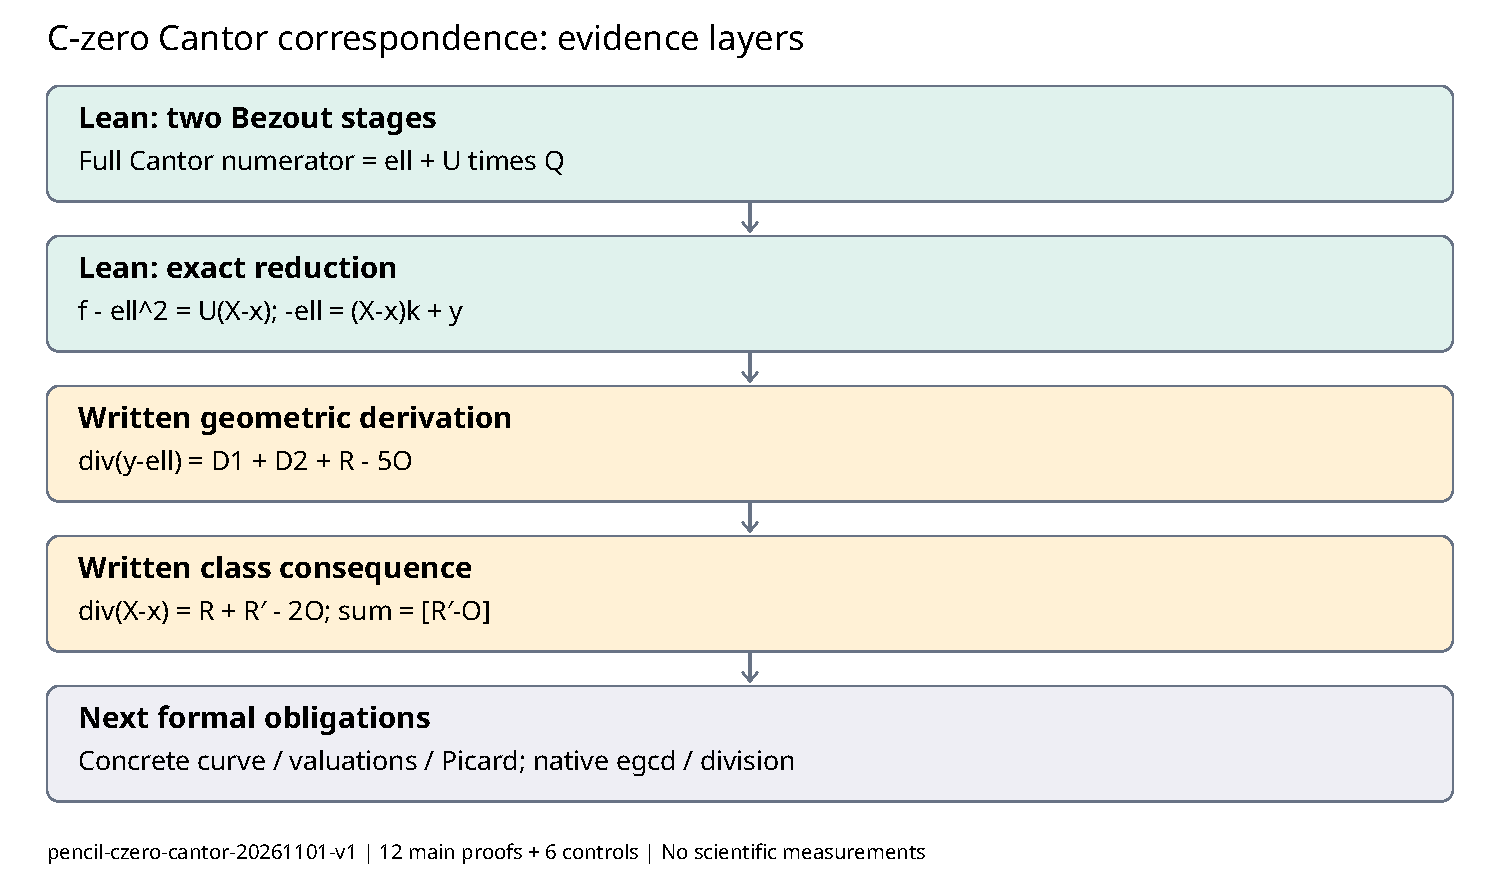
\includegraphics[width=\linewidth]{flow.pdf}
The checked algebra now supplies twelve declarations: CRT composition, a full two-Bezout-stage Cantor numerator identity, monicity and degrees, unique exact quotient, and a negative remainder certificate. These establish the polynomial transition from the two quadratic inputs to the linear output. A separate written geometric derivation below identifies the resulting divisor class under stated smooth-curve assumptions. That geometric derivation is not a Lean theorem.\par\medskip
Checked statement. Let u\_i=X\textasciicircum{}2+q\_i X+r\_i, v\_i=s\_i X+t\_i, a=A/B, ell=v1-a u1=v2-a u2, U=u1u2 and x=q1+q2+a\textasciicircum{}2. Assume a field, monic quintic f with coefficient4 zero, B nonzero, C zero, and u\_i dividing f-v\_i\textasciicircum{}2. Prior checked interpolation proves U divides f-ell\textasciicircum{}2; the imported output theorem gives f-ell\textasciicircum{}2=U(X-x). New Cantor.lean proves -ell=(X-x)k+C(-ell(x)), with k=aX+C(ax+aq1-s1). The initial degree bound is degree ell<=2<4=degree U; the output support is monic of degree1. Unique.lean proves uniqueness of the exact quotient by U. These are exact quotient/remainder certificates, not a replay of native polynomial division.\par\medskip
General composition. Composition.lean allows arbitrary Bezout polynomials e1,e2,c1,c2 satisfying e1u1+e2u2=1 and c1+c2(v1+v2)=1. It proves the literal general Cantor numerator equals ell+U[c1 a(e1+e2)+c2(a\textasciicircum{}2+Q)] when f-ell\textasciicircum{}2=UQ. In particular the second Bezout coefficient c2 need not vanish. Its residue modulo U is ell by the degree bound and uniqueness of polynomial remainder; actual native pegcd/pdiv correctness remains a composition obligation.\par\medskip
Native source correspondence. three\_leads.rs1015--1024 computes aa=dq, bb=dr, cc=-ds, dd=-dt, norm=-B and s1=C. Thus the C=0 branch bypasses the fast nonzero-slope path. Lines1045--1060 execute two pegcd calls, form precisely the numerator in Composition.lean, then call reduce. Lines990--1003 first normalize u and reduce v, then replace u by monic((f-v\textasciicircum{}2)/u) and v by -v modulo new\_u. The certified degrees describe one algebraic iteration: input degree4, output degree1. The proof does not establish native allocation, trim/length equivalence, egcd termination or its word-level Bezout invariant, compiled equivalence, or runtime costs. Source pegcd is at900--926. Source SHA256 and extracted snapshots are in status.json and the manifest.\par\medskip
Written geometric assumptions. Work over an algebraic closure of a field of characteristic not2, on the smooth projective model of y\textasciicircum{}2=f(x), where f is squarefree and monic of degree5. There is a unique infinity point O, with ord\_O(x)=-2 and ord\_O(y)=-5. These local facts and the existence of the smooth projective curve are geometric inputs to this written argument, not assumptions that the desired addition formula holds. Inputs are Mumford divisors obtained from the ideals (u\_i,y-v\_i), with multiplicities defined as local intersection lengths. The equation u\_i divides f-v\_i\textasciicircum{}2 ensures these ideals define finite effective divisors D\_i of degree2. B nonzero makes u1 and u2 coprime, so the two supports do not overlap.\par\medskip
Finite-place multiplicities. Set g=y-ell(x). For a root alpha of f-ell\textasciicircum{}2 with ell(alpha) nonzero, y+ell is a local unit at P=(alpha,ell(alpha)). The identity (y-ell)(y+ell)=f-ell\textasciicircum{}2 shows ord\_P(g) equals the multiplicity of alpha in f-ell\textasciicircum{}2. At a root with ell(alpha)=0, squarefreeness gives f'(alpha) nonzero. Hence f-ell\textasciicircum{}2 has a simple root there. The local parameter y has order1, while x-alpha has order2; ell(x) has order at least2 unless ell is identically zero, and g consequently has order1. These arguments handle ramification and all repeated roots away from ramification, including overlap of the residual root x with a root of U. No assumption of five distinct intersections is used.\par\medskip
Principal divisor calculation. Since degree ell<=2, its pole order at O is at most4, strictly less than the pole order5 of y. Therefore g has exactly a pole of order5 at O, with no leading-term cancellation. The factorization f-ell\textasciicircum{}2=U(X-x), with the finite multiplicity calculation above, gives div(g)=D1+D2+R-5O, where R=(x,ell(x)); this remains an equality of cycles if R already occurs in D1 or D2. For R'=(x,-ell(x)), div(x\_coordinate-x)=R+R'-2O. At a ramification point R=R' the zero has order2, so the same formula holds with multiplicity. Both identities are ordinary principal divisors derived from explicit rational functions.\par\medskip
Passage to actual classes. In the quotient Div0(C)/Prin(C), the first identity gives [D1-2O]+[D2-2O]=-[R-O]. The second gives -[R-O]=[R'-O]. Thus their sum is represented by (X-x,-ell(x)), exactly the certified algebraic output. The argument uses the existing mathematical definition of the Picard/Jacobian quotient; it does not define a bespoke equivalence relation by the desired output rule. For original non-algebraically-closed input fields, all displayed rational functions and Mumford ideals are defined over the original field; one must use its actual Picard scheme or a descent-compatible divisor-class carrier, not silently identify every Galois-fixed class with a rational divisor.\par\medskip
Formal carrier gap. The inspected repository RuntimeSemantics.lean277--302 supplies PrincipalClassInterface with a caller-provided principal-kernel property. ProjectiveLawBoundary.lean179--187 supplies FormulaValid-to-ClassSum as a bridge field. Neither constructs the above curve, valuations, principal divisors or Picard quotient. The scoped search of integration Lean sources and the available partial Mathlib cache found no such implementation. To mechanize the written derivation, implement that geometric carrier, prove infinity orders and local intersection multiplicities, identify Mumford ideals with effective divisors, and descend the two explicit principal divisors to the quotient. This is distinct from the native egcd/division correspondence work.\par\medskip
Checks and retained failures. Final gates: cantor2, unique1, composition1, controls3 and readback1. Six controls cover the explicit rational remainder, wrong sign, wrong abscissa, degree1 output, repeated-root support, and the algebraic identity in characteristic2. Characteristic2 is admitted only by the polynomial identity, not by the geometric y\textasciicircum{}2=f model. The first probe failed because polynomial division names were unavailable in the loaded partial cache; the packet uses certificates rather than claiming those APIs. cantor1 lacked noncomputable on a polynomial constructor; controls1 had indentation errors; controls2 required numeric constant-map normalization. All attempts are retained. No scientific workloads, comparative timing, cohort runs or repository edits were performed. The helper binds direct source/olean roots before and after each check; the transitive dependency cache is a trusted input, not recursively audited here.\par\medskip
Literature and scope. Ozbay Gurler and Hisil, A complete group law on genus-2 Jacobians over any finite field, 2024, sections2.2--2.3, supplies the conventional divisor, principal quotient, Mumford and Cantor definitions: https://link.springer.com/article/10.1007/s13389-024-00351-7 . The original Cantor1987 AMS PDF returned403 and was not inspected. The geometric argument above is supplied explicitly for independent review. This is a producer packet; it does not claim independent review or a mechanized divisor-class theorem.\par\medskip
\end{document}